\chapter{Proverb 12}

\begin{figure}
  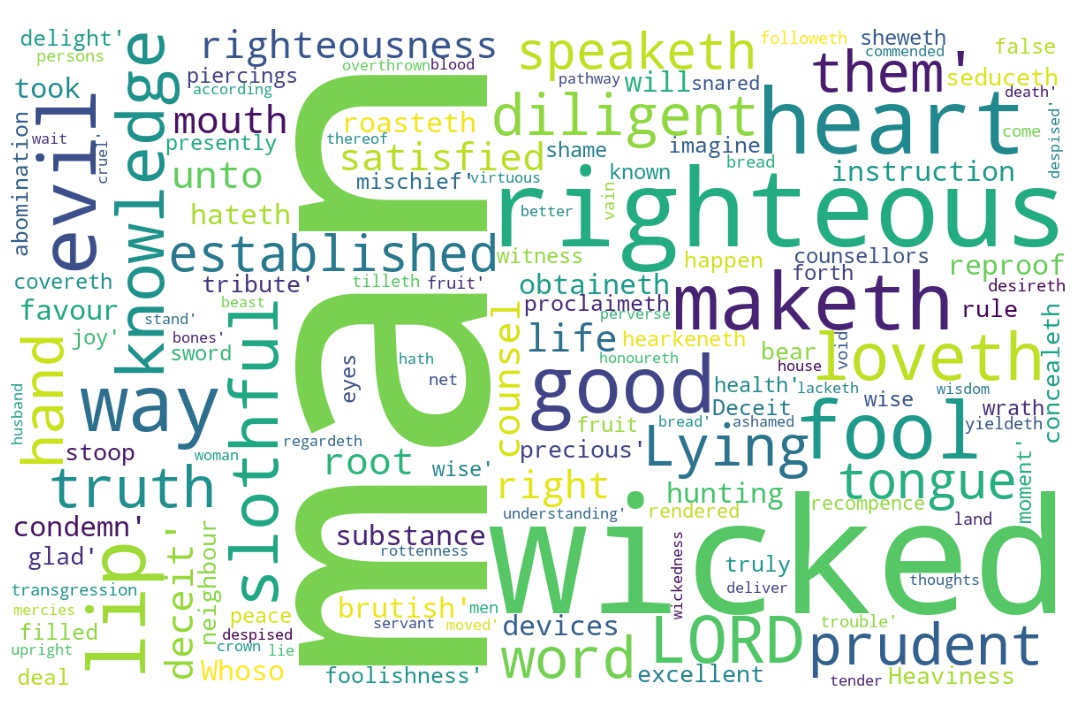
\includegraphics[width=\linewidth]{20OT-Proverbs/Proverb12-WordCloud.jpg}
  \caption{Proverb 12 Word Cloud}
  \label{fig:Proverb 12 Word Cloud}
\end{figure}

\marginpar{\scriptsize \centering \fcolorbox{bone}{lime}{\textbf{SURE THINGS}}\\ (Proverb 12:1-27) \begin{compactenum}[I.][8]
    \item \textbf{Contented Man} \index[scripture]{Proverbs!Pro 12:01}(Pro 12:1) 
    \item \textbf{Contentious Mate} \index[scripture]{Proverbs!Pro 12:04}(Pro 12:4) 
    \item \textbf{Commended Man} \index[scripture]{Proverbs!Pro 12:08}(Pro 12:8) 
    \item \textbf{Condemned Man} \index[scripture]{Proverbs!Pro 12:09}(Pro 12:9) 
    \item \textbf{Correct Mouth} \index[scripture]{Proverbs!Pro 12:17}(Pro 12:17) 
    \item \textbf{Continual Misery} \index[scripture]{Proverbs!Pro 12:25}(Pro 12:25) 
    \item \textbf{Comforting Materials} \index[scripture]{Proverbs!Pro 12:27}(Pro 12:27) 
\end{compactenum}}

\marginpar{\scriptsize \centering \fcolorbox{bone}{yellow}{\textbf{WICKED WAYS \& WORDS}}\\ (Proverb 12:1-27) \begin{compactenum}[I.][8]
    \item They do not Provide \textbf{Security} \index[scripture]{Proverbs!Pro 12:03}(Pro 12:3) 
    \item They do not Provide \textbf{Satisfaction} \index[scripture]{Proverbs!Pro 12:11}\index[scripture]{Proverbs!Pro 12:14}(Pro 12:11, 14) 
    \item They are \textbf{Snares} \index[scripture]{Proverbs!Pro 12:13}(Pro 12:13) 
    \item They lead to \textbf{Shame} \index[scripture]{Proverbs!Pro 12:16}(Pro 12:16) 
    \item They Pierce like a \textbf{Sword} \index[scripture]{Proverbs!Pro 12:18}(Pro 12:18) 
    \item They Produce \textbf{Slothfulness and Servanthood} \index[scripture]{Proverbs!Pro 12:24}\index[scripture]{Proverbs!Pro 12:27}(Prov 12:24, 27) 
\end{compactenum}}

\marginpar{\scriptsize \centering \fcolorbox{bone}{black}{\textbf{\textcolor[cmyk]{0,0,0,0}{PARTS OF LIFE}}}\\ (Proverb 12:1-27) 
 \begin{compactenum}[I.][8]
    \item \textbf{Path to Growth} \index[scripture]{Proverbs!Pro 12:01}(Pro 12:1) 
    \item \textbf{Promise of God} \index[scripture]{Proverbs!Pro 12:02} (Pro 12:2) 
    \item \textbf{Perennial Aggravation} \index[scripture]{Proverbs!Pro 12:04}(Pro 12:04)
    \item \textbf{Perverse Goals} \index[scripture]{Proverbs!Pro 12:08}(Pro 12:08) 
    \item \textbf{Presence of Grief} \index[scripture]{Proverbs!Pro 12:08}(Pro 12:08)
    \item \textbf{Practical Regard} \index[scripture]{Proverbs!Pro 12:10}(Pro 12:10) 
    \item \textbf{Pattern of Goodness} \index[scripture]{Proverbs!Pro 12:24}(Pro 12:24) 
\end{compactenum}}


\marginpar{\scriptsize \centering \fcolorbox{bone}{blue}{\textbf{\textcolor[cmyk]{0,0,0,0}{A VIRTUOUS WOMAN}}}\\ (Proverb 12:1-27) 
 \begin{compactenum}[I.][8]
    \item \textbf{Correctable} \index[scripture]{Proverbs!Pro 12:04}(Pro 12:4) 
    \item \textbf{Conformable} \index[scripture]{Proverbs!Pro 12:04}(Pro 12:4) 
    \item \textbf{Cooperative} \index[scripture]{Proverbs!Pro 12:04}(Pro 12:4) 
    \item \textbf{Calm} \index[scripture]{Proverbs!Pro 12:04}(Pro 12:4) 
    \item A \textbf{Crown} \index[scripture]{Proverbs!Pro 12:04}(Pro 12:4) 
    \item \textbf{Caring} \index[scripture]{Proverbs!Pro 12:04}(Pro 12:4) 
    \item \textbf{Considerate} \index[scripture]{Proverbs!Pro 12:04}(Pro 12:4) 
\end{compactenum}}

\marginpar{\scriptsize \centering \fcolorbox{bone}{orange}{\textbf{THE EXAMINATION}}\\ (Proverb 12:1-27) \begin{compactenum}[I.][8]
    \item What their \textbf{Hearts} Love \index[scripture]{Proverbs!Pro 12:01}(Pro 12:1) 
    \item What Their \textbf{Hands} Produce \index[scripture]{Proverbs!Pro 12:04}(Pro 12:4) 
    \item \textbf{How} they treat the Helpless \index[scripture]{Proverbs!Pro 12:08}(Pro 12:8) 
    \item The \textbf{Health} of Their speech \index[scripture]{Proverbs!Pro 12:181}(Pro 12:8) 
    \item What he \textbf{Hearkened} to \index[scripture]{Proverbs!Pro 12:15}(Pro 12:15) 
    \item What is \textbf{Honoured} to \index[scripture]{Proverbs!Pro 12:09}(Pro 12:9) 
    \item How they \textbf{Handle} the Details
    \index[scripture]{Proverbs!Pro 12:09}(Pro 12:9) 
\end{compactenum}}

%%%%%%%%%%%%%%%%%%%%%%%%%%%%%%%%%%
%%%%%%%%%%%%%%%%%%%%%%%%%%%%%%%%%
\footnote{\textcolor[cmyk]{0.99998,1,0,0}{\hyperlink{TOC}{Return to end of Table of Contents.}}}\footnote{\href{https://audiobible.com/bible/proverbs_12.html}{\textcolor[cmyk]{0.99998,1,0,0}{Proverbs Audio}}}\textcolor[cmyk]{0.99998,1,0,0}{Whoso \fcolorbox{bone}{lime}{loveth instruction} loveth \fcolorbox{bone}{blue}{\textbf{\textcolor[cmyk]{0,0,0,0}{knowledge}}}: but he that hateth reproof \emph{is} brutish.}
[2] \textcolor[cmyk]{0.99998,1,0,0}{A good \emph{man} obtaineth \fcolorbox{bone}{lime}{favour of} \fcolorbox{bone}{blue}{\textbf{\textcolor[cmyk]{0,0,0,0}{the LORD}}}: but \fcolorbox{bone}{bone}{a} man of wicked devices will he condemn.}
[3] \textcolor[cmyk]{0.99998,1,0,0}{A man shall \fcolorbox{bone}{yellow}{not be}  \fcolorbox{bone}{yellow}{established} by wickedness: but the root of the righteous shall not be moved.}
[4] \textcolor[cmyk]{0.99998,1,0,0}{A virtuous woman \emph{is} \fcolorbox{bone}{bone}{a} crown to her husband: but she that maketh ashamed \emph{is} as \fcolorbox{bone}{blue}{\textbf{\textcolor[cmyk]{0,0,0,0}{rottenness in his bones}}}.}
[5] \textcolor[cmyk]{0.99998,1,0,0}{The thoughts of the righteous \emph{are} right: \emph{but} the counsels of the wicked \emph{are} deceit.}
[6] \textcolor[cmyk]{0.99998,1,0,0}{The words of the wicked \emph{are} to lie in wait for blood: but the mouth of the upright shall deliver them.}
[7] \textcolor[cmyk]{0.99998,1,0,0}{The wicked are overthrown, and \emph{are} not: but the house of the righteous shall stand.}
[8] \textcolor[cmyk]{0.99998,1,0,0}{A man shall be \fcolorbox{bone}{lime}{commended} according to his wisdom: but he that is of \fcolorbox{bone}{bone}{a} \fcolorbox{bone}{blue}{\textbf{\textcolor[cmyk]{0,0,0,0}{perverse}}} heart shall be despised.}
[9] \textcolor[cmyk]{0.99998,1,0,0}{\emph{He} \emph{that} \emph{is} \fcolorbox{bone}{lime}{despised}, and hath \fcolorbox{bone}{bone}{a} servant, \emph{is} better than he that honoureth himself, and lacketh bread.}
[10] \textcolor[cmyk]{0.99998,1,0,0}{A righteous \emph{man} \fcolorbox{bone}{blue}{\textbf{\textcolor[cmyk]{0,0,0,0}{regardeth}}} the life of his beast: but the tender mercies of the wicked \emph{are} cruel.}
[11] \textcolor[cmyk]{0.99998,1,0,0}{He that tilleth his land shall be \fcolorbox{bone}{yellow}{satisfied} with bread: but he that followeth vain \emph{persons} \emph{is} void of \fcolorbox{bone}{MYGOLD}{understanding}.}
[12] \textcolor[cmyk]{0.99998,1,0,0}{The wicked desireth the net of evil \emph{men}: but the root of the righteous yieldeth \emph{fruit}.}
[13] \textcolor[cmyk]{0.99998,1,0,0}{The wicked is \fcolorbox{bone}{yellow}{snared} by the \fcolorbox{bone}{MYGOLD}{transgression} of \emph{his} lips: but the just shall come out of trouble.}\footnote{\textbf{Ecclesiastes 9:12} - For man also knoweth not his time: as the fishes that are taken in an evil net, and as the birds that are caught in the snare; so are the sons of men snared in an evil time, when it falleth suddenly upon them.}\footnote{\textbf{Isaiah 28:13} - But the word of the LORD was unto them precept upon precept, precept upon precept; line upon line, line upon line; here a little, and there a little; that they might go, and fall backward, and be broken, and snared, and taken.}\footnote{\textbf{Isaiah 42:22} - But this is a people robbed and spoiled; they are all of them snared in holes, and they are hid in prison houses: they are for a prey, and none delivereth; for a spoil, and none saith, Restore.}
[14] \textcolor[cmyk]{0.99998,1,0,0}{A man shall be satisfied with good by the fruit of \emph{his} mouth: and the recompence of \fcolorbox{bone}{bone}{a} man's hands shall be rendered unto him.}
[15] \textcolor[cmyk]{0.99998,1,0,0}{The way of \fcolorbox{bone}{bone}{a} fool \emph{is} right in his own eyes: but he that hearkeneth unto counsel \emph{is} wise.}
[16] \textcolor[cmyk]{0.99998,1,0,0}{A fool's wrath is presently known: but \fcolorbox{bone}{bone}{a} prudent \emph{man} covereth \fcolorbox{bone}{yellow}{shame}.}\footnote{\textbf{Proverb 27:3}  -  A stone is heavy, and the sand weighty; but a fool’s wrath is heavier than them both.}
[17] \textcolor[cmyk]{0.99998,1,0,0}{\emph{He} \emph{that} \fcolorbox{bone}{lime}{speaketh truth} sheweth forth \fcolorbox{bone}{MYGOLD}{righteousness}: but \fcolorbox{bone}{bone}{a} false witness deceit.}
[18] \textcolor[cmyk]{0.99998,1,0,0}{There is that speaketh like the piercings of \fcolorbox{bone}{bone}{a} \fcolorbox{bone}{yellow}{sword}: but the tongue of the wise \emph{is} health.}
[19] \textcolor[cmyk]{0.99998,1,0,0}{The lip of truth shall be established for ever: but \fcolorbox{bone}{bone}{a} lying tongue \emph{is} but for \fcolorbox{bone}{bone}{a} moment.}
[20] \textcolor[cmyk]{0.99998,1,0,0}{Deceit \emph{is} in the heart of them that imagine evil: but to the counsellors of peace \emph{is} joy.}
[21] \textcolor[cmyk]{0.99998,1,0,0}{There shall no evil happen to the just: but the wicked shall be filled with mischief.}
[22] \textcolor[cmyk]{0.99998,1,0,0}{Lying lips \emph{are} abomination to the LORD: but they that deal truly \emph{are} his delight.}
[23] \textcolor[cmyk]{0.99998,1,0,0}{A prudent man concealeth knowledge: but the heart of fools proclaimeth foolishness.}
[24] \textcolor[cmyk]{0.99998,1,0,0}{\fcolorbox{bone}{blue}{\textbf{\textcolor[cmyk]{0,0,0,0}{The hand of the diligent}}} shall bear rule: but the \fcolorbox{bone}{yellow}{slothful} shall be under \fcolorbox{bone}{yellow}{tribute.}}
[25] \textcolor[cmyk]{0.99998,1,0,0}{\fcolorbox{bone}{lime}{Heaviness} in the heart of man maketh it stoop: but \fcolorbox{bone}{bone}{a} good word maketh it glad.}
[26] \textcolor[cmyk]{0.99998,1,0,0}{The righteous \emph{is} more excellent than his neighbour: but the way of the wicked seduceth them.}
[27] \textcolor[cmyk]{0.99998,1,0,0}{The \fcolorbox{bone}{yellow}{slothful} \emph{man} roasteth not that which he took in hunting: but the substance of \fcolorbox{bone}{bone}{a} diligent man \emph{is} \fcolorbox{bone}{lime}{precious}.}
[28] \textcolor[cmyk]{0.99998,1,0,0}{In the way of \fcolorbox{bone}{MYGOLD}{righteousness} \emph{is} life; and \emph{in} the pathway \emph{thereof} \emph{there} \emph{is} no death.}\footnote{\textbf{Psalm 1:1, 6} - Blessed is the man that walketh not in the counsel of the ungodly, nor standeth in the way of sinners, nor sitteth in the seat of the scornful. [6] For the LORD knoweth the way of the righteous: but the way of the ungodly shall perish.}




